%
% teil1.tex -- Beispiel-File für das Paper
%
% (c) 2020 Prof Dr Andreas Müller, Hochschule Rapperswil
%
\section{Fraktale
\label{ifs:section:teil1}}
\rhead{Problemstellung}
Bevor wir die IFS genauer ansehen, schauen wir uns Fraktale genauer an.


Über die genaue Definition von Fraktalen sind sich die Mathematiker nicht einig. 
In diesem Kapitel orientieren wir uns an den Eigenschaften welche Kenneth Falconer in seinem Buch Fractal Geometry \cite{ifs:fractal-geometry} beschreibt.
Von einem Fraktal $F$ können wir folgende Eigenschaften erwarten:
\begin{enumerate}
	\item $F$ hat eine unendlich feine Struktur
	\item $F$ kann nicht mit der klassischen Geometrie beschrieben werden.
	\item Oftmals haf $F$ eine Form von Selbstähnlichkeit.
	\item Die 'fraktale Dimension' ist grösser als die Topologische Dimension
	\item Viele Fraktale lassen sich einfach beschrieben
\end{enumerate}
\subsection{Koch Kurve
	\label{ifs:subsection:lilkoch}}
Diese Eigenschaften möchten wir nun anhand der Koch Kurve näher anschauen.
In \ref{ifs:kochkurve8} sehen wir die Koch Kurve. Wie man schon erahnen kann, besteht sie aus lauter kleineren Kopien von sich selber. 
Den Konstruktionsvorgang ist in Abbildung \ref{ifs:kochconst} dargestellt.
Gestartet wird mit einer einzelnen Strecke der Länge $a$.
Diese wird in ersten Schritt mit vier gleich langen Streckenabschnitte der Länge $\frac{a}{3}$ ersetzt.
In \ref{ifs:kochconstb} ist die Anordnung dieser vier Streckenabschnitte ersichtlich. 
Dieser Schritt wird nun für jeden der resultierten Streckenabschnitten wiederholt.
Die Kurve besteht also aus vier kleineren Kopien von der ganzen Kurve, was auch unter Selbstähnlichkeit bekannt ist.


\begin{figure}
	\centering
	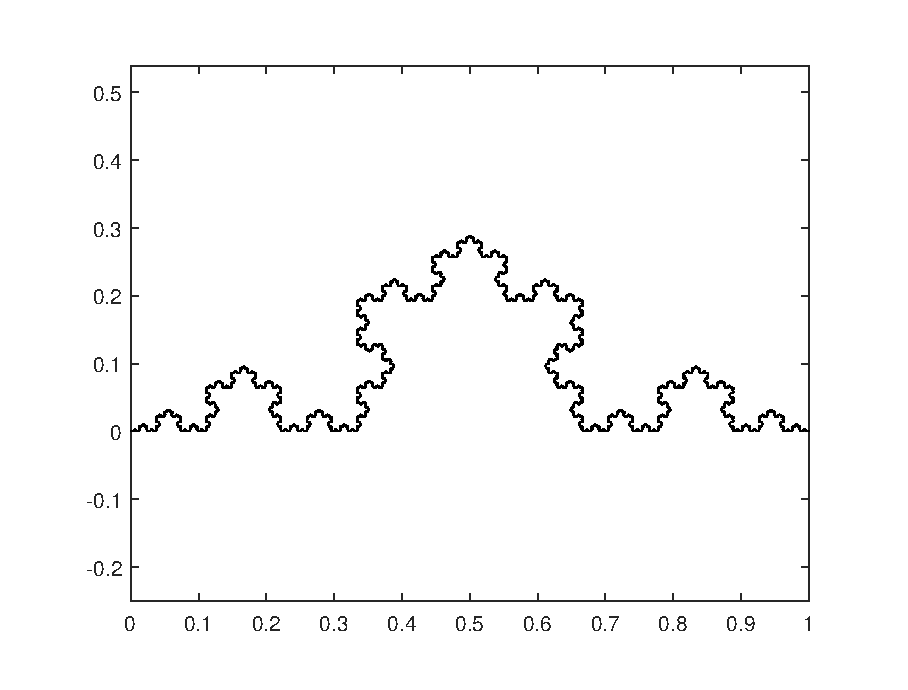
\includegraphics{papers/ifs/images/koch8}
	\caption{Koch Kurve}
	\label{ifs:kochkurve8}
\end{figure}

\begin{figure}
	\centering
	\subfigure[]{
		\label{ifs:kochconsta}
		\includegraphics[width=0.32\textwidth]{papers/ifs/images/koch0}}
	\subfigure[]{
		\label{ifs:kochconstb}
		\includegraphics[width=0.32\textwidth]{papers/ifs/images/koch1}} 
	\subfigure[]{
		\label{kochconstc}
		\includegraphics[width=0.32\textwidth]{papers/ifs/images/koch2}}
	\caption{(a) Start (b) 1. Iteration (c) 2. Iteration}
	\label{ifs:kochconst}
\end{figure}

Die resultierende Kurve hat ein paar interessante Eigenschaften.
Die Länge der Kurve lasst sich einfach berechnen.
\begin{align*}
	l_0 = a ,\quad l_1 = a  \frac{4}{3} ,\quad l_2 = a  \left( \frac{4}{3}\right)^2 , \quad ... , \quad
	l_n = a * \left( \frac{4}{3}\right)^n \quad
	\Rightarrow \quad
	\lim_{n\to\infty} a  \left( \frac{4}{3}\right)^n = \infty
\end{align*}
In jedem Schritt wird die Länge um den Faktor $\frac{4}{3}$ verlängert. Somit divergiert die Länge gegen Unendlich. 
Die Fläche unter der Kurve lässt sich folgendermassen berechnen
\begin{align*}
	A_0 = 0 , \quad A_1 = \left( \frac{a}{3}\right)^2 \frac{\sqrt{3}}{4} = a^2 \frac{\sqrt{3}}{36}\\
	A_2 = A_1 + 4\left( \frac{a}{3^2}\right)^2 \frac{\sqrt{3}}{4} = A_1 + \frac{4}{9} A_1 \\ 
	A_3 = A_1 + A_2 + 4^2 \left( \frac{a}{3^2}\right)^2 \frac{\sqrt{3}}{4} = A_1 + \frac{4}{9} A_1 + \left( \frac{4}{9}\right)^2 A_1	 
\end{align*}
Wir sehen, dass mit jedem Schritt die neu dazugekommene Fläche um $\frac{4}{9}$ kleiner ist.
Daraus resultiert eine konvergierende Geometrische Reihe.
\begin{align*}
	A_n = A_1 \sum_{i = 0}^{n-1} \left( \frac{4}{9}\right)^n =  a^2 \frac{\sqrt{3}}{36} \sum_{i = 0}^{n-1} \left( \frac{4}{9}\right)^n \\
	\lim_{n\to\infty} a^2 \frac{\sqrt{3}}{36} \sum_{i = 0}^{n-1} \left( \frac{4}{9}\right)^n = \frac{\sqrt{3}}{20} a^2
\end{align*}
Wie wir sehen ist die Kochkurve ein Konstrukt mit endlicher Fläche, aber unendlichem Umfang.
Zu guter Letzt bestimmen wir die Dimension der Kurve. 
Es gibt viele verschiedene Arten die Dimension zu definieren. Diese können dann auch unterschiedliche Resultate liefern.
Vor allem im Zusammenhang mit Fraktalen findet man in der Literatur viele verschiedene Arten.
In diesem Beispiel werden wir die Ähnlichkeits-Dimension \cite{ifs:fractal-geometry}.
\begin{align*}
	D = - \frac{log(N)}{log(\epsilon)}
\end{align*}
Mit ihr kann man einfach die Dimension selbstähnlicher Mengen bestimmen.
Als Beispiel nehmen wir ein gleichseitiges Dreieck. Dieses besteht aus $N = 4$ Kopien mit halber ($\epsilon = 1/2$) Kantenlänge.
Somit hat das Dreieck die Dimension $D = 2$.
Die Koch Kurve besteht aus $N = 4$ Kopien mit Kantenlänge $\epsilon = 1/3$.
\begin{align*}
	D = - \frac{log(N)}{log(\epsilon)} = - \frac{log(4)}{log(1/3)} \approx 1.2619
\end{align*}
Wie wir nun sehen besitzt die Kochkurve alle oben beschriebenen Eigenschaften von Fraktalen. 
Dies muss jedoch nicht bei allen Fraktalen der Fall. Sonst wäre die Frage nach einer 'richtigen' Definition einfach zu beantworten.

